
\documentclass[12pt,a4paper, oneside]{extreport}

%%%%%%%%%% Математика %%%%%%%%%%
\usepackage{amsmath,amsfonts,amssymb,amsthm,mathtools}
% Показывать номера только у тех формул, на которые есть \eqref{} в тексте.
%\mathtoolsset{showonlyrefs=true}
%\usepackage{leqno} % Нумерация формул слева
%\usepackage{tipa} %Для формулки из логитов


\usepackage{hyphenat}

%%%%%%%%%% Шрифты %%%%%%%%
\usepackage[english, russian]{babel} % выбор языка для документа
\usepackage[utf8]{inputenc} % задание utf8 кодировки исходного tex файла
\usepackage[X2,T2A]{fontenc}        % кодировка

\usepackage{fontspec}         % пакет для подгрузки шрифтов
\setmainfont{Times New Roman}       % задаёт основной шрифт документа

\usepackage{unicode-math}      % пакет для установки математического шрифта
%\setmathfont{Asana-Math.otf}    % шрифт для математики

% Конкретный символ из конкретного шрифта
% \setmathfont[range=\int]{Neo Euler}


%%%%%%%%%% Работа с картинками %%%%%%%%%
\usepackage{graphicx}                  % Для вставки рисунков
\usepackage{graphics}
\graphicspath{{images/}{pictures/}}    % можно указать папки с картинками
\usepackage{wrapfig}                   % Обтекание рисунков и таблиц текстом


%%%%%%%%%% Работа с таблицами %%%%%%%%%%
\usepackage{tabularx}            % новые типы колонок
\usepackage{tabulary}            % и ещё новые типы колонок
\usepackage{array,delarray}      % Дополнительная работа с таблицами
\usepackage{longtable}           % Длинные таблицы
\usepackage{multirow}            % Слияние строк в таблице
\usepackage{float}               % возможность позиционировать объекты в нужном месте

\usepackage{booktabs}            % таблицы как в книгах

% Заповеди из документации к booktabs:
% 1. Будь проще! Глазам должно быть комфортно
% 2. Не используйте вертикальные линни
% 3. Не используйте двойные линии. Как правило, достаточно трёх горизонтальных линий
% 4. Единицы измерения - в шапку таблицы
% 5. Не сокращайте .1 вместо 0.1
% 6. Повторяющееся значение повторяйте, а не говорите "то же"
% 7. Есть сомнения? Выравнивай по левому краю!

%  вычисляемые колонки по tabularx
\newcolumntype{C}{>{\centering\arraybackslash}X}
\newcolumntype{L}{>{\raggedright\arraybackslash}X}
\newcolumntype{Y}{>{\arraybackslash}X}
\newcolumntype{Z}{>{\centering\arraybackslash}X}


%%%%%%%%%% Графика и рисование %%%%%%%%%%
\usepackage{tikz, pgfplots}      % язык для рисования графики из latex'a

%%%%%%%%%% Гиперссылки %%%%%%%%%%
\usepackage{xcolor}              % разные цвета

\usepackage{hyperref}
\hypersetup{
	unicode=true,           % позволяет использовать юникодные символы
	colorlinks=true,       	% true - цветные ссылки, false - ссылки в рамках
	urlcolor =blue,         % цвет ссылки на url
	linkcolor=black,        % внутренние ссылки
	citecolor=black,        % на библиографию
	breaklinks              % если ссылка не умещается в одну строку, разбивать ли ее на две части?
}


%%%%%%%%%% Другие приятные пакеты %%%%%%%%%
\usepackage{multicol}       % несколько колонок
\usepackage{verbatim}       % для многострочных комментариев
\usepackage{cmap} % для кодировки шрифтов в pdf

\usepackage{enumitem} % дополнительные плюшки для списков
%  например \begin{enumerate}[resume] позволяет продолжить нумерацию в новом списке

\usepackage{todonotes} % для вставки в документ заметок о том, что  осталось сделать
% \todo{Здесь надо коэффициенты исправить}
% \missingfigure{Здесь будет Последний день Помпеи}
% \listoftodos --- печатает все поставленные \todo'шки



%%%%%%%%%%%%%% ГОСТОВСКИЕ ПРИБАМБАСЫ %%%%%%%%%%%%%%%

%%% размер листа бумаги
\usepackage[paper=a4paper,top=15mm, bottom=15mm,left=35mm,right=10mm,includehead]{geometry}


\usepackage{setspace}
\setstretch{1.5}     % Межстрочный интервал
\setlength{\parindent}{1.25cm} % Красная строка.


%\flushbottom       % Эта команда заставляет LaTeX чуть растягивать строки, чтобы получить идеально прямоугольную страницу
\righthyphenmin=2  % Разрешение переноса двух и более символов
\widowpenalty=10000  % Наказание за вдовствующую строку (одна строка абзаца на этой странице, остальное --- на следующей)
\clubpenalty=10000  % Наказание за сиротствующую строку (омерзительно висящая одинокая строка в начале страницы)
\tolerance=1000     % Ещё какое-то наказание.


% Нумерация страниц сверху по центру
\usepackage{fancyhdr}
\pagestyle{fancy}
%\fancyhead{ } % clear all fields
%\fancyfoot{ } % clear all fields
\fancyhf{}
\fancyhead[R]{Касьянова Ксения (СМАР19)}
\fancyfoot[C]{\thepage}
% Чтобы не прорисовывалась черта!
\renewcommand{\headrulewidth}{0pt}


% Нумерация страниц с надписью "Глава"
\usepackage{etoolbox}
\patchcmd{\chapter}{\thispagestyle{plain}}{\thispagestyle{fancy}}{}{}


%%% Заголовки
\usepackage[indentfirst]{titlesec}{\raggedleft}
% Заголовки по левому краю
% опция identfirst устанавливает отступ в первом абзаце



% В Linux этот пакет сделан косячно. Исправляет это следующий непонятный кусок кода.
\makeatletter
\patchcmd{\ttlh@hang}{\parindent\z@}{\parindent\z@\leavevmode}{}{}
\patchcmd{\ttlh@hang}{\noindent}{}{}{}
\makeatother


% Редактирования Глав и названий
\titleformat{\chapter}
{\normalfont\large\bfseries}
{\thechapter }{0.5 em}{}

% Редактирование ненумеруемых глав chapter* (Введение и тп)
\titleformat{name=\chapter,numberless}
{\centering\normalfont\bfseries\large}{}{0.25em}{\normalfont}

% Убирает чеканутые отступы вверху страницы
\titlespacing{\chapter}{0pt}{-\baselineskip}{\baselineskip}

% Более низкие уровни
\titleformat{\section}{\bfseries}{\thesection}{0.5 em}{}
\titleformat{\subsection}{\bfseries}{\thesubsection}{0.5 em}{}

\titlespacing*{\section}{0 pt}{\baselineskip}{\baselineskip}
\titlespacing*{\subsection}{0 pt}{\baselineskip}{\baselineskip}


% Содержание. Команды ниже изменяют отступы и рисуют точечки!
\usepackage{titletoc}

\titlecontents{chapter}
[1em] %
{\normalsize}
{\contentslabel{1 em}}
{\hspace{-1 em}}
{\normalsize\titlerule*[10pt]{.}\contentspage}

\titlecontents{section}
[3 em] %
{\normalsize}
{\contentslabel{1.75 em}}
{\hspace{-1.75 em}}
{\normalsize\titlerule*[10pt]{.}\contentspage}

\titlecontents{subsection}
[6 em] %
{\normalsize}
{\contentslabel{3 em}}
{\hspace{-3 em}}
{\normalsize\titlerule*[10pt]{.}\contentspage}


% Правильные подписи под таблицей и рисунком
% Документация к пакету на русском языке!
\usepackage[tableposition=top, singlelinecheck=false]{caption}
\usepackage{subcaption}


\DeclareCaptionStyle{base}%
[justification=centering,indention=0pt]{}
\DeclareCaptionLabelFormat{gostfigure}{Рисунок #2}
\DeclareCaptionLabelFormat{gosttable}{Таблица #2}

\DeclareCaptionLabelSeparator{gost}{~---~}
\captionsetup{labelsep=gost}

\DeclareCaptionStyle{fig01}%
[margin=5mm,justification=centering]%
{margin={3em,3em}}
\captionsetup*[figure]{style=fig01,labelsep=gost,labelformat=gostfigure,format=hang}

\DeclareCaptionStyle{tab01}%
[margin=5mm,justification=centering]%
{margin={3em,3em}}
\captionsetup*[table]{style=tab01,labelsep=gost,labelformat=gosttable,format=hang}


% межстрочный отступ в таблице
\renewcommand{\arraystretch}{1.2}



% многостраничные таблицы под РОССИЙСКИЙ СТАНДАРТ
% ВНИМАНИЕ! Обязательно за CAPTION !
\usepackage{fr-longtable}



%Более гибкие спсики
\usepackage{enumitem}
% сообщаем окружению о том, что существует такая штук как нумерация русскими буквами.
\makeatletter
\AddEnumerateCounter{\asbuk}{\russian@alph}{щ}
\makeatother


%%% ГОСТОВСКИЕ СПИСКИ

% Первый тип списков. Большая буква.
\newlist{Enumerate}{enumerate}{1}

\setlist[Enumerate,1]{labelsep=0.5em,leftmargin=1.25em,labelwidth=1.25em,
	parsep=0em,itemsep=0em,topsep=0ex, before={\parskip=-1em},label=\arabic{Enumeratei}.}


% Второй тип списков. Маленькая буква.
\setlist[enumerate]{label=\arabic{enumi}),parsep=0em,itemsep=0em,topsep=0.75ex, before={\parskip=-1em}}


% Третий тип списков. Два уровня.
\newlist{twoenumerate}{enumerate}{2}
\setlist[twoenumerate,1]{itemsep=0mm,parsep=0em,topsep=0.75ex,, before={\parskip=-1em},label=\asbuk{twoenumeratei})}
\setlist[twoenumerate,2]{leftmargin=1.3em,itemsep=0mm,parsep=0em,topsep=0ex, before={\parskip=-1em},label=\arabic{twoenumerateii})}


% Четвёртый тип списков. Список с тире.
\setlist[itemize]{label=--,parsep=0em,itemsep=0em,topsep=0ex, before={\parskip=-1em},after={\parskip=-1em}}


%%% WARNING WARNING WARNIN!
%%% Если в списке предложения, то должна по госту стоять точка после цифры => команда Enumerate! Если идет перечень маленьких фактов, не обособляемых предложений то после цифры идет скобка ")" => команда enumerate! Если перечень при этом ещё и двууровневый, то twoenumerate.




%%%%%%%%%% Список литературы %%%%%%%%%%

%\usepackage[%
%backend=biber, %подключение пакета biber (тоже нужен)
%bibstyle=gost-numeric, %подключение одного из четырех главных стилей biblatex-gost
%sorting=ntvy, %тип сортировки в библиографии
%]{biblatex}

\usepackage[backend=biber,style=gost-numeric, maxbibnames=9,maxcitenames=2,uniquelist=false, babel=other]{biblatex}



% Справка по 4 главным стилям для ленивых:
% gost-inline  ссылки внутри теста в круглых скобках
% gost-footnote подстрочные ссылки
% gost-numeric затекстовые ссылки
% gost-authoryear тоже затекстовые ссылки, но немного другие

% Подробнее смотри страницу 4 документации. Она на русском.

% Ещё немного настроек
\DeclareFieldFormat{postnote}{#1} %убирает с. и p.
\renewcommand*{\mkgostheading}[1]{#1} % только лишь убираем курсив с авторов


\addbibresource{diploma11.bib} % сюда нужно вписать свой bib-файлик.



% Этот кусок кода выносит русские источники на первое место. Костыль описали авторы пакета в руководстве к нему. Подробнее смотри:
% https://github.com/odomanov/biblatex-gost/wiki/Как-сделать%2C-чтобы-русскоязычные-источники-предшествовали-остальным
\DeclareSourcemap{
	\maps[datatype=bibtex]{
		\map{
			\step[fieldsource=langid, match=russian, final]
			\step[fieldset=presort, fieldvalue={a}]
		}
		\map{
			\step[fieldsource=langid, notmatch=russian, final]
			\step[fieldset=presort, fieldvalue={z}]
		}
	}
}

\DefineBibliographyStrings{english}{%
	pages = {P\adddot},
	number = {№},
}



\begin{document} % Начала документа



%%%%%%%%%%%%%%%%%%%% ВВЕДЕНИЕ %%%%%%%%%%%%%%%%%%%%%%%%%%%%%%%%%%%%
\section*{Анализ влияния завершения инвестиционных программ в электроэнергетике на \\ экономику РФ в рамках модели IS-LM-BP}

\subsection*{Описание ситуации}
Во-первых, в связи с завершением инвестиционных программ в 2018-2019 гг в электроэнергетике, в отрасли высвобождается около 1,5 трлн рублей, которые можно реинвестировать в модернизацию. Стабильный операционный денежный поток от платежей по ДПМ\footnote{ Договор на предоставление мощности (ДПМ) — обязательство инвестора построить и ввести в эксплуатацию  новые генерирующие мощности в обмен на повышенную стоимость производимых мощностей на 10 лет. } в 2018–2020 годах не приведет к росту инвестиций в данный период, а новые инвестиционные проекты находятся на стадии разработки \cite{ID5, ID3}. Ожидается, что инвестиционная пауза в отрасли продлится до начала 2020-х годов \cite{ID7}

По завершении инвестиционной деятельности введены новые генерирующие мощности,  содержание которых гораздо затратнее, чем старых, так как при модернизации использовались зарубежные газовые турбины большой мощности (в России такого оборудования пока нет) \cite{ID1}.

Ввод в эксплуатацию в 2018–2022 годах АЭС суммарной мощностью 3,5 ГВт станет основным драйвером роста цен на электроэнергию в секторе генерации выше инфляции.
Удержать цены на электроэнергию в пределах инфляции невозмощно  (даже в случае ужесточения тарифного регулирования) с 2017-го по 2020-й вряд ли удастся, так как на рост цены в том числе влияет и повышение цен на топливо \cite{ID7}.

\subsection*{Анализ события в рамках IS-LM-BP}
Пусть в начальном состоянии $A$ экономика находится в равновесии.

Инвестиции в развитие отечественной электроэнергетики обусловлены необходимостью модернизации отрасли в условиях стремительно устаревающих мощностей, поэтому их можно отнести к автономным, т.е. не зависящим от ставки процента. Результатом завершения инвестиционных программ (до введения новых) в 2019 году будет снижение автономных инвестиций, а следовательно и  снижение автономных расходов.

\begin{equation}\label{key}
\Delta A_0 =  \Delta AE_0 = \Delta I_0  < 0.
\end{equation}

Необходимость использования зарубежного оборудования, в т.ч. для ремонта приведет к росту импорта, однако будем считать, что закупки импортного оборудования были произведены ранее, т.е. равновесное состояние уже учитывает это изменение, а ремонт пока не требуется, поэтому  импорт останется фиксированным. 

В условиях активной политики таргетирования инфляции тарифная политика в отношении регулируемых цен на электричество будет ограничительной, поэтому в рамках данного анализа будем считать, что в целом влияние на общий уровень цен нивелируется за счет государственного регулирования рынка. Учитывая, что из-за невозможности "хранения" электроэнергии предложение можно считать неэластичным по цене, поэтому для простоты будем считать, что влияние на равновесие на этом рынке в результате регулирования незначительно в масштабах всей экономики. Уровень цен будем считать постоянным, изменения реального спроса на деньги и номинального предложения в рамках  анализа влияния данного события мы не рассматриваем, поэтому в результате кривая $LM$ останется на месте.

Итак, в результате снижения инвестиций кривая $IS$ сдвигается  влево и экономика переходит из состояния $A$ в состояние промежуточного равновесия $B$.
В этом состоянии выпуск и ставка процента ниже исходных, но оно не является равновесным, так как еще не установлено равновесие платежного баланса.
Снижение производства отрицательно влияет на счет текущих операций, с ростом импорта  спрос на отечественную валюту падает. Со снижением ставки отечественный капитал становится менее привлекательным для инвесторов. 
При условии плавающего валютного курса и слабой мобильности капитала изменение счета текущих операций по модулю  больше изменения счета движения капитала, поэтому в точке $B$ результате имеем потенциальную  возможность возникновения положительного сальдо платежного баланса, в результате курс начинает расти, что сокращает экспорт и увеличивает импорт, а кривая $IS$ сдвигается еще левее и экономика переходит в равновесное состояние $C$, что проиллюстрировано на рисунке 1.

\begin{equation}\label{key}
\begin{rcases}
\Delta Y < 0 \rightarrow \Delta Im < 0 \rightarrow  \Delta CA > 0  \\
\Delta R < 0  \rightarrow \Delta CF < 0 
\end{rcases} \Rightarrow \Delta (CA-CF) >0.
\end{equation}


\begin{figure}
	\centering
	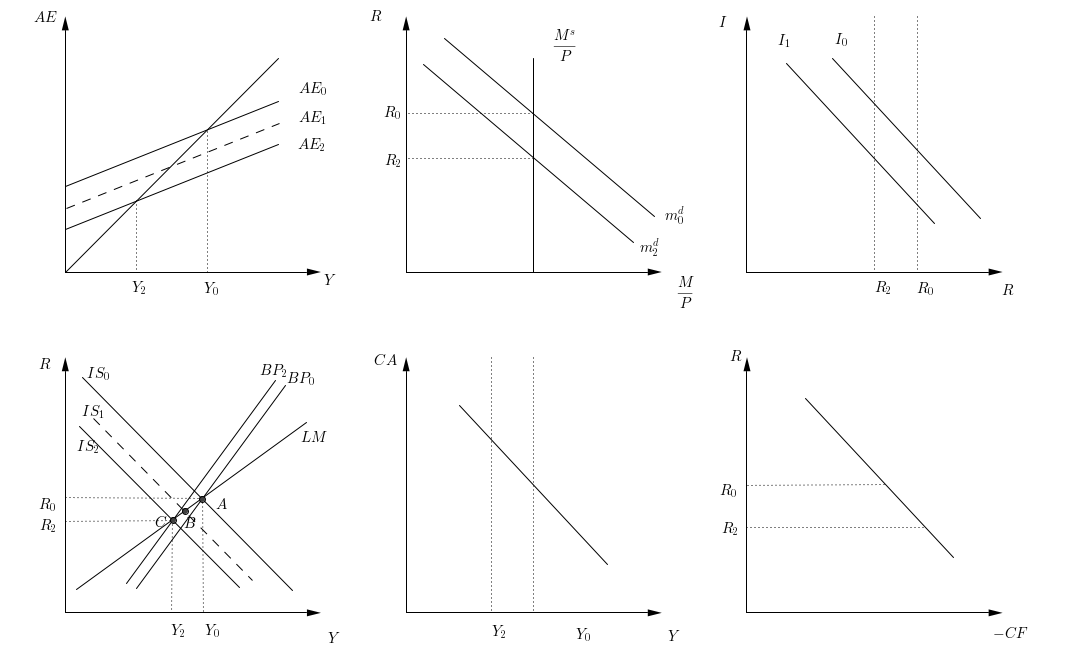
\includegraphics[width=1\linewidth]{screenshot002}
	\caption{}
	\label{fig:screenshot002}
\end{figure}




\subsection*{Практические рекомендации}

%Данный анализ отражает влияние шока инвестиций на экономику в рамках модели IS-LM-BP, однако надо понимать, что для упрощения мы предполагаем, что данное событие параллельно не повлияло ни на  импорт, ни на цены, так как делать какие-то выводы о совокупном влиянии на ставку и выпуск при сдвиге сразу всех кривых не представляется возможным без эмпирических оценок параметров модели.

В рамках нашей модели, получаем, что снижение автономных инвестиций привело к снижению равновесного выпуска, снижению реальной ставки, росту курса. 


Предположим, что государство  хочет  нивелировать изменения, вызванные снижением автономных инвестиций  с помощью  фискальной  политики, поскольку  в условиях плавающего валютного курса и слабой мобильности капитала она будет более   эффективна, чем монетарная. 
Произойдет обратная ситуация (за исключением сдвига кривой инвестиций), как показано на рисунке 2. 

\begin{figure}
	\centering
	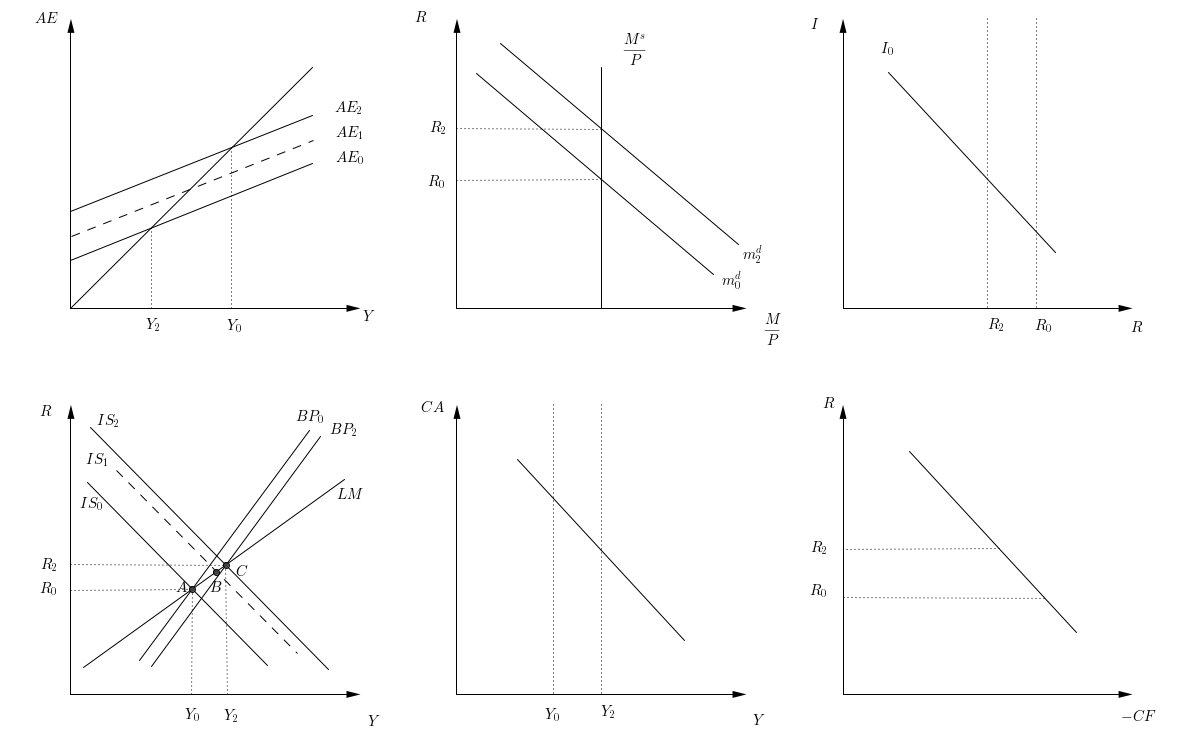
\includegraphics[width=1\linewidth]{screenshot003}
	\caption{}
	\label{fig:screenshot003}
\end{figure}



Увеличив госзакупки на ту же величину, на которые снизились автономные инвестиции экономика вернется в первоначальное состояние.  Но   с 2020-х годов планируется запуск новых инвестиционных проектов. Это событие приведет к сдвигу кривой IS вправо, поэтому при необходимости  величину госзакупок можно скорректировать исходя из доступной информации о планируемой величине инвестиций.  
Так же предполагается, что в при  развитии программ импортозамещения в области разработки и производства генерирующего оборудования можно будет добиться снижения импорта, однако это процесс длительный и маловероятно, что он  произойдет уже в следующем году \cite{ID5}. 


Данный анализ отражает общие тенденции возникшие в результате  шока инвестиций на экономику в рамках модели IS-LM-BP, однако надо понимать, что для упрощения мы предполагаем, что данное событие происходит при прочих равных, а экономика изначально находится в равновесии, что на самом деле может быть не так. 

%параллельно не повлияло ни на  импорт, ни на цены, так как делать какие-то выводы о совокупном влиянии на ставку и выпуск при сдвиге сразу всех кривых не представляется возможным без эмпирических оценок параметров модели.





%%%%%%%%%%% Список литературы	%%%%%%%%%%%


\nocite{*}  %Чтобы в список литературы напечаталичь все источники из bib-файла

% Если нам хочется, чтобы в списке литературы были не полуторные интервалы можно воспользоваться следующим приёмом:
\begingroup
\setstretch{1}
\addcontentsline{toc}{chapter}{Список литературы}
\printbibliography[title = {Список литературы}]
\endgroup



%%%%%%%%%%%%%%%%%%%% Приложения %%%%%%%%%%%%%%%%%%%%

\appendix
\renewcommand{\thechapter}{\Asbuk{chapter}}

%%%%%%%%%% titlesec для приложений
\titleformat{\chapter}
 {\normalfont\bfseries\large}{\chaptertitlename~\thechapter}{0.25em}{\normalfont}



\end{document}
